% 图 2.6 自旋 1/2 磁矩的能量随磁场的变化：m_j=±1/2 两支，劈裂 g*mu_B*B
\documentclass[tikz,border=5pt]{standalone}
\usetikzlibrary{arrows.meta}
\usepackage{amsmath}
\usepackage{bm}
\usepackage{fontspec}
\setmainfont{Times New Roman}
\begin{document}
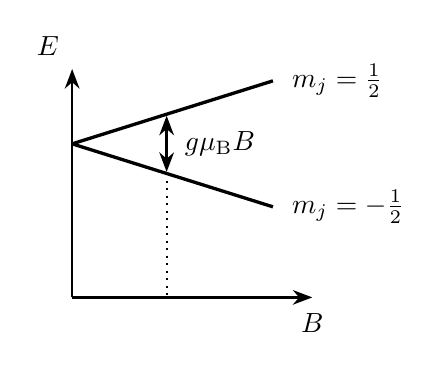
\begin{tikzpicture}[line width=0.8pt,>=Stealth]
% 坐标轴
\draw[->,line width=0.9pt] (0.3,0.25) -- (0.3,3.15) node[above left=1pt] {$E$};
\draw[->,line width=0.9pt] (0.3,0.25) -- (3.35,0.25) node[below=2pt] {$B$};
% 两支能级（起点在 E 轴上，斜率对称：E = ± mu_B B）
\draw[line width=1.2pt] (0.3,2.20) -- (2.85,3.00) node[right=3pt] {$m_j=\frac{1}{2}$};
\draw[line width=1.2pt] (0.3,2.20) -- (2.85,1.40) node[right=3pt] {$m_j=-\frac{1}{2}$};
% g*mu_B*B 双箭头与虚线
\draw[dotted,line width=0.7pt] (1.5,1.8235) -- (1.5,0.25);
\draw[<->,line width=0.9pt] (1.5,1.8435) -- (1.5,2.5565);
\node[right=2pt] at (1.53,2.20) {$g\mu_{\mathrm{B}}B$};
\end{tikzpicture}
\end{document}
